\section{FFS}
% TODO: Fix this section in relation to what the email comments said on march 8th
The artifact that will be developed as a result of this thesis is the Fejk FileSystem (FFS). It uses online services to store the data but behaves as a mountable filesystem for the users. The filesystem will be minimal and not support all functionalities that other filesystems do, such as links. The reasoning is that these behaviors are not required for a useable system, and when comparing the system to distributed filesystems such as Google Drive, many of these other filesystems also often do not support links.

Figure~\ref{fig:ffs_inode_diag} presents the basic outline of FFS and a example content of the filesystem. FFS is based on the idea of inode filesystems but instead of an inode pointing to specific blocks in a disk, the inodes of FFS will instead keep track of the id numbers of the posts on the online services where the file is located. 

As a deniable filesystem, you should not be able to gain any information about the filesystem without the correct credentials. Using incorrect credentials, the filesystem will just show an empty filesystem meaning that the adversary will know if the credentials provided are correct and that the filesystem is empty, or if the credentials were incorrect. Only when the correct credentials are provided will FFS show the filesystem of the user.

\begin{figure}[!ht]
	\begin{center}
	  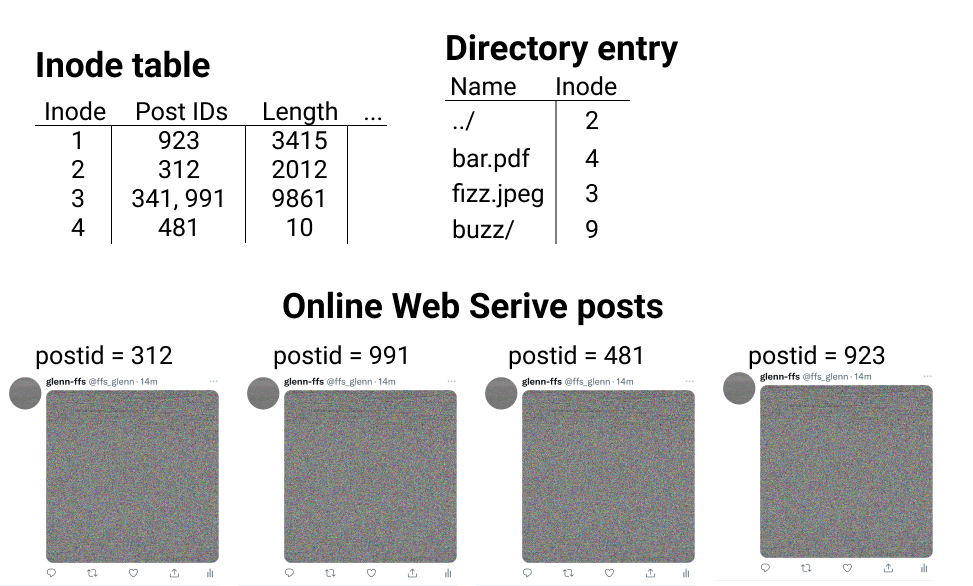
\includegraphics[width=0.8\textwidth]{figures/ffs_inode_diagram.png}
	\end{center}
	\caption{Basic structure of FFS inode-based structure}
	\label{fig:ffs_inode_diag}
\end{figure}

% TODO: add about how FFS will use a inode table (FAT?) instead of a linked list like in SocialStegDisc